In introductory courses, we start with linear predictors since it is easy to understand. Low dimensional linear regression is what statisticians worked in back in the early days, where data was generally low dimensional.\footnote{Quoting Larry Wasserman, even 5 dimensions was considered high and 10 was considered massive. } Generally, we had $d < n$, but these days, we are in the regime where $d > n$. For example, in genetic data, you could have a sample of $n = 100$ people but each of them have genetic sequences at $d = 10^6$. When the dimensions become high, the original methods of linear regression tend to break down, which is why I separate low and high dimensional linear regression. The line tends to be fuzzy between these two regimes, but we will not worry about strictly defining that now. Let's introduce the most general variant of linear regression. 

\begin{definition}[Linear Regression Model]
  A \textbf{linear regression model} is a probabilistic model that predicts the conditional distribution of $y$ given $x$ as 
  \begin{equation}
    y = b + w^T x + \epsilon
  \end{equation}
  Another common and compact way of writing it is to encode $x$ as a $(d+1)$-dimensional vector where $x_0 = 1$, and write 
  \begin{equation}
    y = \beta^T x + \epsilon, \beta = (b, w) \in \mathbb{R}^{d+1}
  \end{equation}
  Get used to both methods. It has the following assumptions. 
  \begin{enumerate}
    \item \textit{Linearity in Parameters}. Note that this does not mean linearity in the \textit{covariates}.\footnote{Therefore you could build a regression using non-linear transformations of the covariates, for instance, $y = w_1 x_1 + w_2 x_2^2 + w_3 \log(x_1)$. }
    \item \textit{Weak exogeneity}. The covariates are observed without error. 
    \item $\epsilon$ is $0$-mean. 
    \item \textit{Homoscedasticity}: $\epsilon$ has constant variance. 
    \item The $\epsilon$'s are uncorrelated with each other. 
    \item \textit{No multicolinearity}: There exists no covariates that are perfectly correlated. 
  \end{enumerate}
\end{definition} 

Let's go through these assumptions in detail.  

\textit{Linearity}: This is pretty straightforward, but many beginners assume that we must only fit \textit{lines} with respect to the covariates $x_i$. This is not true (consider polynomial regression), and all we are assuming is linearity with respect to the \textit{parameters}. 

In fact, we can consider combinations of fixed nonlinear functions of the input variables of the form
\begin{equation}
  f(x, w) = w_0 + \sum_{j=1}^{M-1} w_j \phi_j (x) = \beta^T \phi(x)
\end{equation}
where each \textit{basis function} $\phi_j: \mathbb{R}^D \longrightarrow \mathbb{R}$. If you need to further relax the assumption, you are better off using non-linear modeling. 

\begin{example}[Basis Functions]
  We can choose many different types of basis functions. The following examples are for 1-dimensional $x$. 
  \begin{enumerate}
    \item The \textit{polynomial basis functions} form powers of $x$ such that
    \begin{equation}
      \phi_j (x) = x^j
    \end{equation}
    One limitation of polynomial basis function is that they are global functions on the input variable, so that changes in one region of input space affect all other regions. This can be resolved by dividing up the input space up into regions and fit a different polynomial in each region, leading to \textit{spline functions}.

    \item The \textit{Gaussian basis functions} (which can be, but not necessarily must be interpreted in the probabilistic way), have the form
    \begin{equation}
      \phi_j (x) = \exp \bigg(-\frac{(x - \mu_j)^2}{2 s^2}\bigg)
    \end{equation}
    where the $\mu_j$ govern the locations of the basis functions in input space, and the parameter $s$ governs their spatial scale.

    \item The \textit{sigmoidal basis functions} are of form
    \begin{equation}
      \phi_j (x) = \sigma \bigg( \frac{x - \mu_j}{s} \bigg), \text{ where } \sigma(a) = \frac{1}{1 + e^{-a}}
    \end{equation}
    Rather than using the sigmoid function $\sigma$, we could also use the hyperbolic tangent $\text{tanh}(a) = 2\sigma(a) - 1$.

    \item The \textit{Fourier basis functions} leads to an expansion in sinusoidal functions, which has specific frequency and infinite spatial extent. By contrast, basis functions that are localized to finite regions of input space necessarily comprise a spectrum of different spatial frequencies. In many signal processing applications, it is of interest to consider basis functions that are localized in both space and frequency, leading to a class of functions known as \textit{wavelets}.
  \end{enumerate}

  \begin{figure}[H]
    \centering
    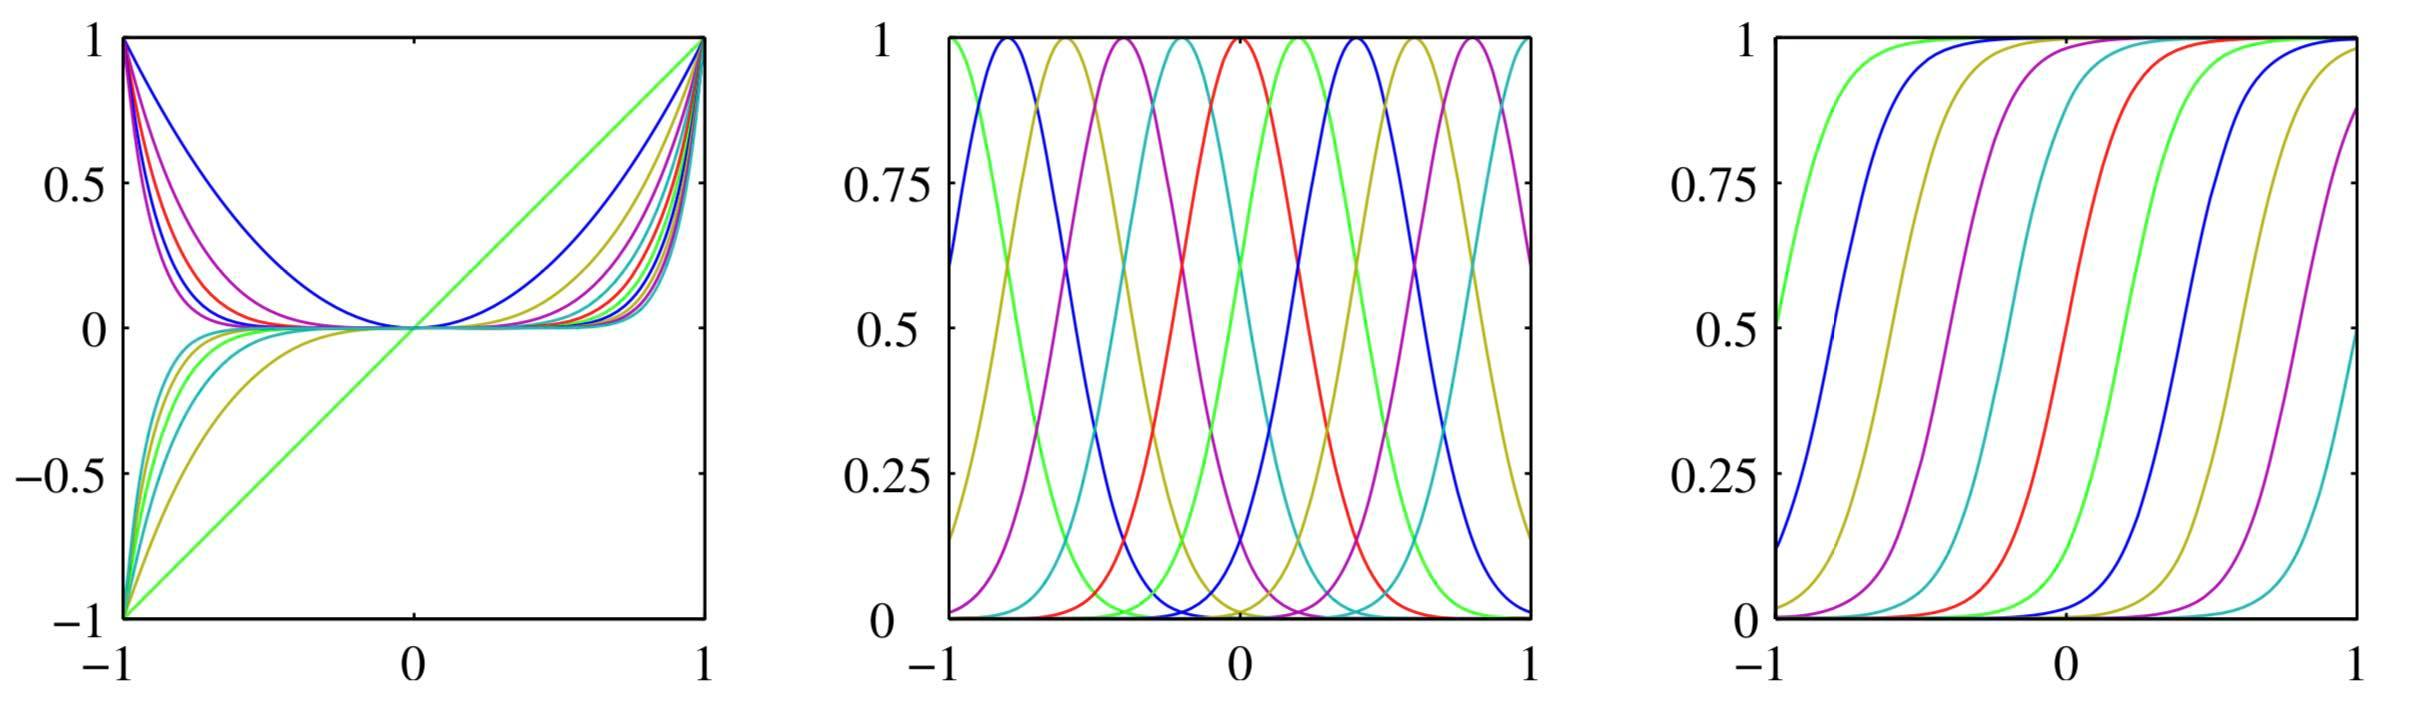
\includegraphics[width=0.9\textwidth]{img/Linear_basis_functions.jpg}
    \caption{Different types of basis functions}
  \end{figure}
\end{example}

\textit{Weak exogeneity}: The sensitivity of the model can be tested to the assumption of weak exogeneity by doing bootstrap sampling for the covariates and seeing how the sampling affects the parameter estimates. Covariates measured with error used to be a difficult problem to solve, as they required errors-in-variables models, which have very complicated likelihoods. In addition, there is no universal fitting library to deal with these. But nowadays, with the availability of Markov Chain Monte Carlo (MCMC) estimation through probabilistic programming languages, it is a lot easier to deal with these using Bayesian hierarchical models (or multilevel models, or Bayesian graphical models---these have many names).

\textit{Constant variance}: the simplest fix is to do a variance-stabilising transformation on the data. Assuming a constant coefficient of variation rather than a constant mean could also work. Some estimation libraries (such as the \verb+glm+ package in R) allow specifying the variance as a function of the mean.

\textit{Independence of errors}: this is dangerous because in fields like finance, things are usually highly correlated in times of crisis. The most important thing is to understand how risky this assumption is for your setting. If necessary, add a correlation structure to your model, or do  a multivariate regression. Both of these require significant resources to estimate parameters, not only in terms of computational power but also in the amount of data required. Another field that looks for correlation between samples is time series analysis, which we will get to in another set of notes. 

\textit{No Multicollinearity}. Assume that two variables are perfectly correlated. Then, there would be pairs of parameters that are indistinguishable if moved in a certain linear combination. This means that the variance of $\hat{\boldsymbol{\beta}}$ will be very ill conditioned, and you would get a huge standard error in some direction of the $\beta_i$'s. We can fix this by making sure that the data is not redundant and manually removing them, standardizing the variables, or making a change of basis to remove the correlation. If we just leave the model as is, numerical problems might occur depending on how the fitting algorithms invert the matrices involved. The t-tests that the regression produces can no longer be trusted.\footnote{I suggest reading this Wikipedia article on multicollinearity, as it contains useful information: \url{https://en.wikipedia.org/wiki/Multicollinearity}. Multicollinearity is a favorite topic of discussion for quant interviewers, and they usually have strong opinions about how it should be handled. The model's intended use will determine how sensitive it is to ignoring the error distribution. In many cases, fitting a line using least-squares estimation is equivalent to assuming errors have a normal distribution. If the real distribution has heavier tails, like the t-distribution, how risky will it make decisions based on your outputs? One way to address this is to use a technique like robust-regression. Another way is to think about the dynamics behind the problem and which distribution would be best suited to model them---as opposed to just fitting a curve through a set of points.} 

In order to check multicollinearity, we compute the correlation matrix, and see if there are any off-diagonal entries that are very close to $1$, then there is multicollinearity. 

Some more terminology: \textbf{multiple linear regression} assumes that we have several covariates and one response. If we extend this to multiple responses (i.e. a response vector), this is called \textbf{multivariate linear regression}. The simple case for one response is called \textbf{simple linear regression}, and we will mention some nice formulas and intuition that come out from working with this. 

